\section{Fits at higher sensitivity}
\label{app:high_sensitivity_fits}
This appendix includes 2D data fits with the reactor constraint applied, with contours up to $3\sigma$ confidence level and the corresponding comparisons with MaCh3\cite{MaCh3:2018}.

\subsection{Results for \main}
In \cref{fig:dcp_vs_ssqth23_data_3sigma} the result for \main with reactor constraint is shown.

\begin{figure*}[htb]
	\center
	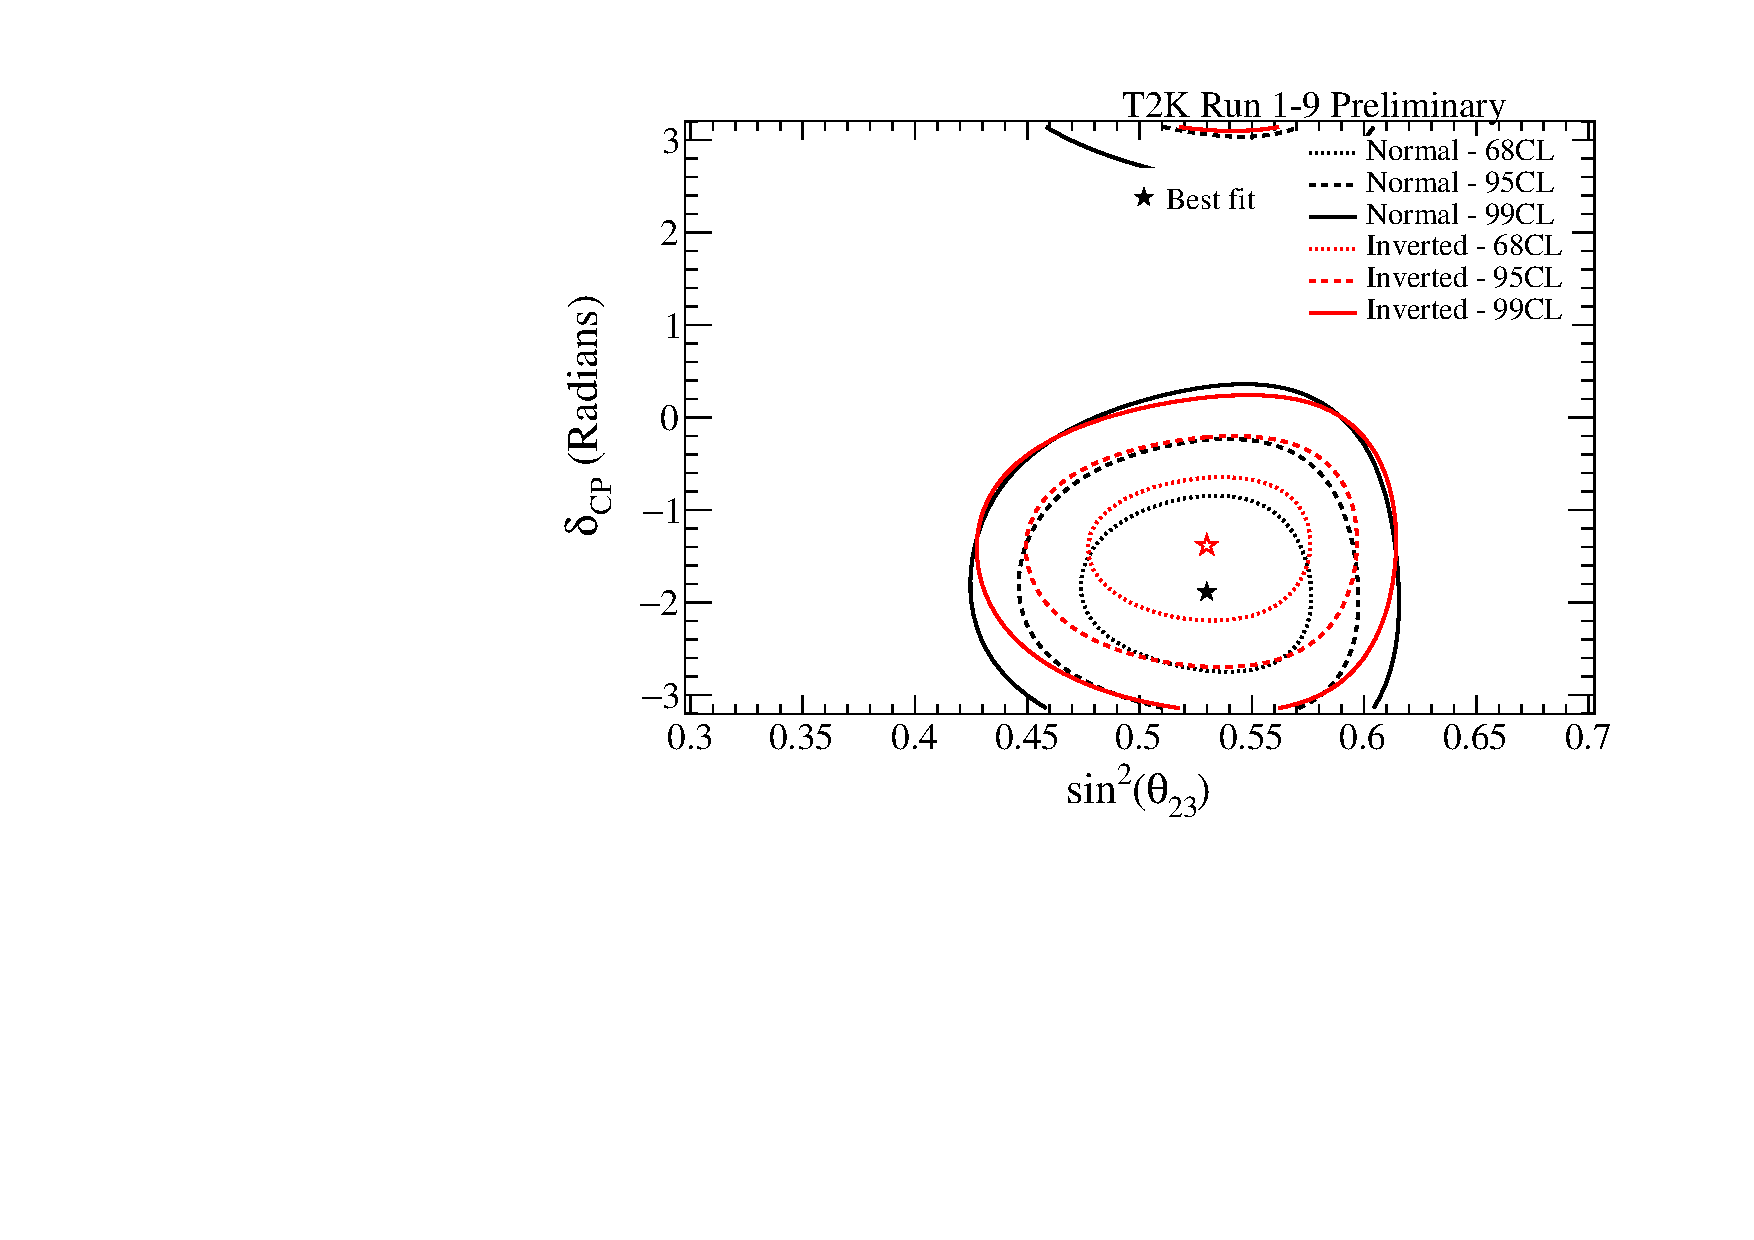
\includegraphics[width=0.45\textwidth]{images/data/3sigma/mixing23_deltacp_data_reactor_global_3sigma}
	\caption {
		Contours at 68\%, 95\% and 99\% CL for \main with reactor constraint. Normal and inverted hierarchy contours are independent. All 5 samples were used to produce these fits.
	}
	\label{fig:dcp_vs_ssqth23_data_3sigma}
\end{figure*}

\subsection{Results for \appearance}
In \cref{fig:ssqth13_vs_dcp_data_3sigma} the result for \appearance with reactor constraint is shown.

\begin{figure*}[htb]
	\center
	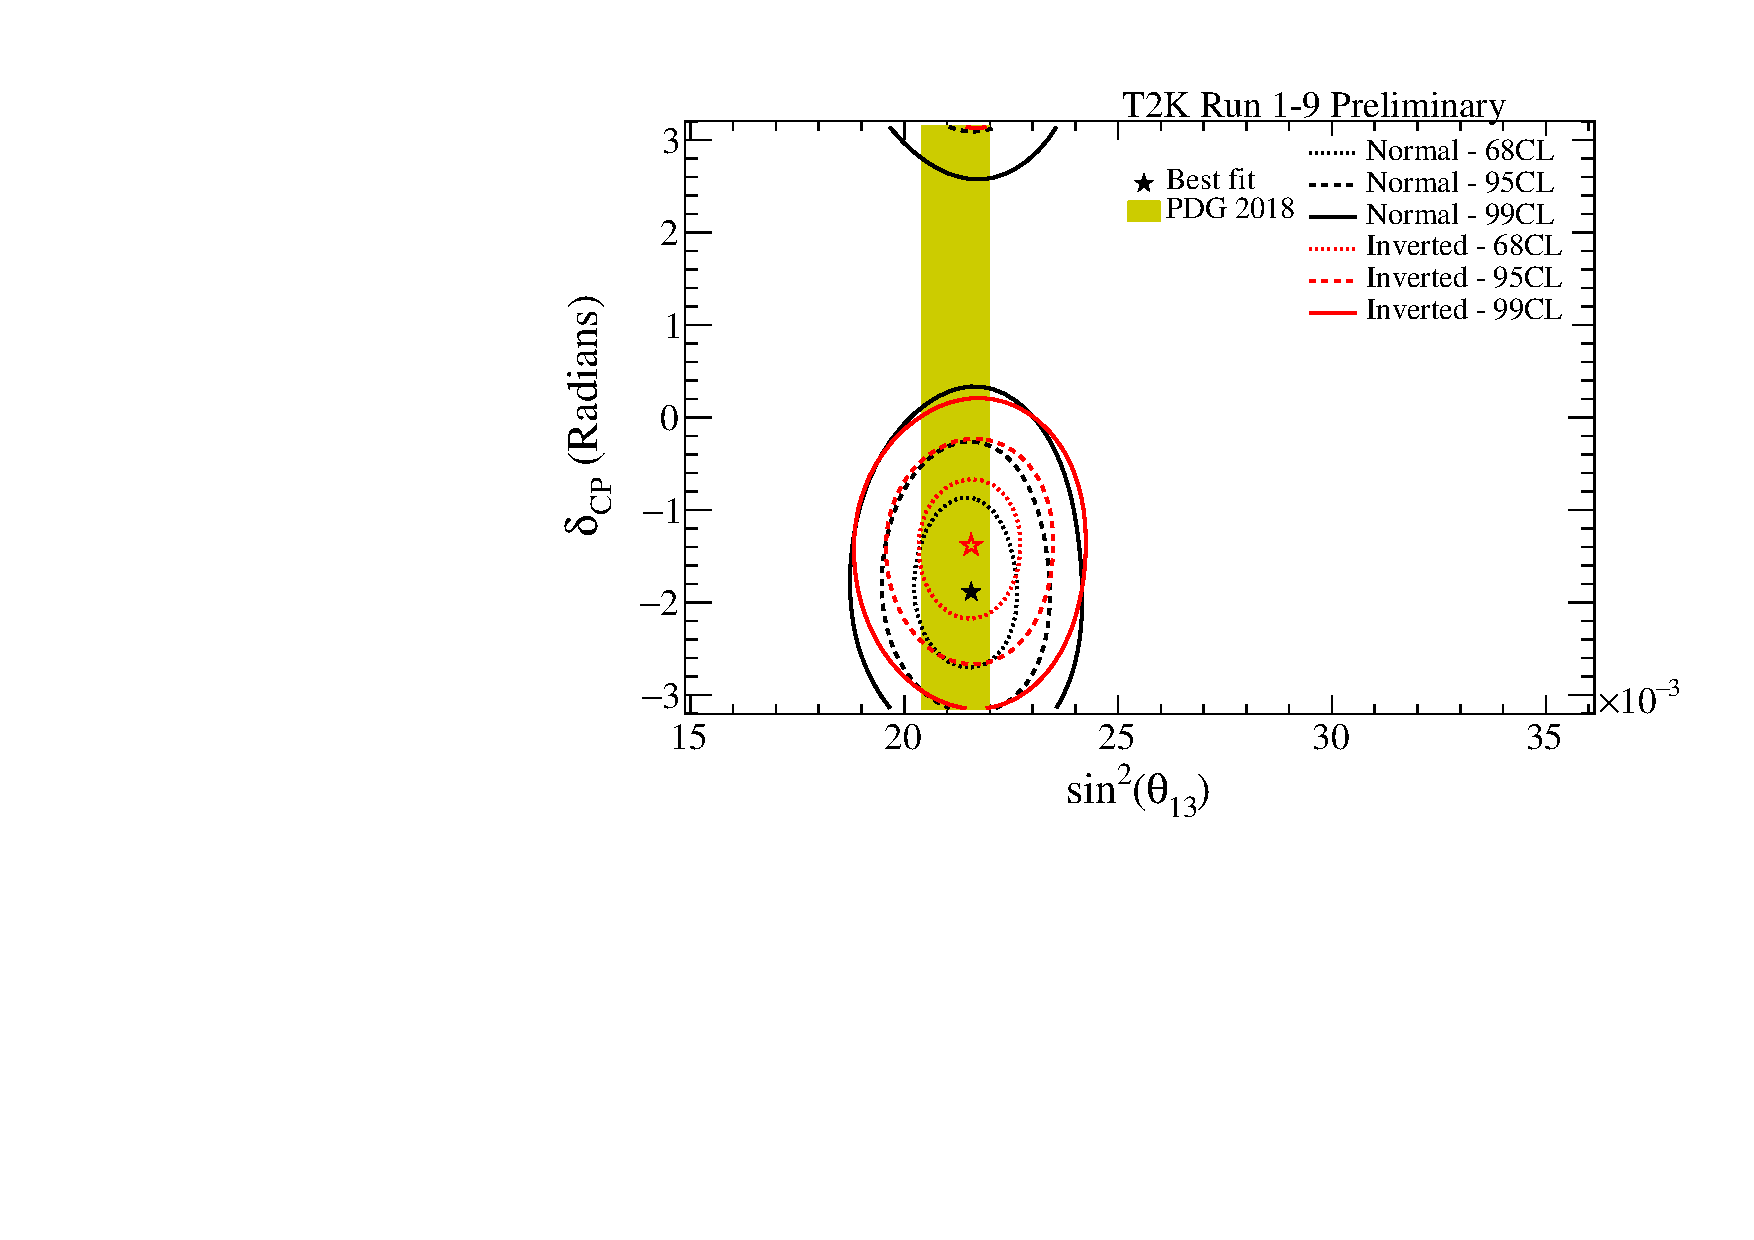
\includegraphics[width=0.45\textwidth]{images/data/3sigma/mixing13_deltacp_data_reactor_global_3sigma}
	\caption {
		Contours at 68\%, 95\% and 99\% CL for \appearance with reactor constraint. Normal and inverted hierarchy contours are independent. All 5 samples were used to produce these fits.
	}
	\label{fig:ssqth13_vs_dcp_data_3sigma}
\end{figure*}
\clearpage

\subsection{Results for \disappearance}

The result for \disappearance with reactor constraint is shown in fig.~\ref{fig:ssqth23_vs_dmsq23_data_3sigma}.

\begin{figure*}[htb]
	\center
	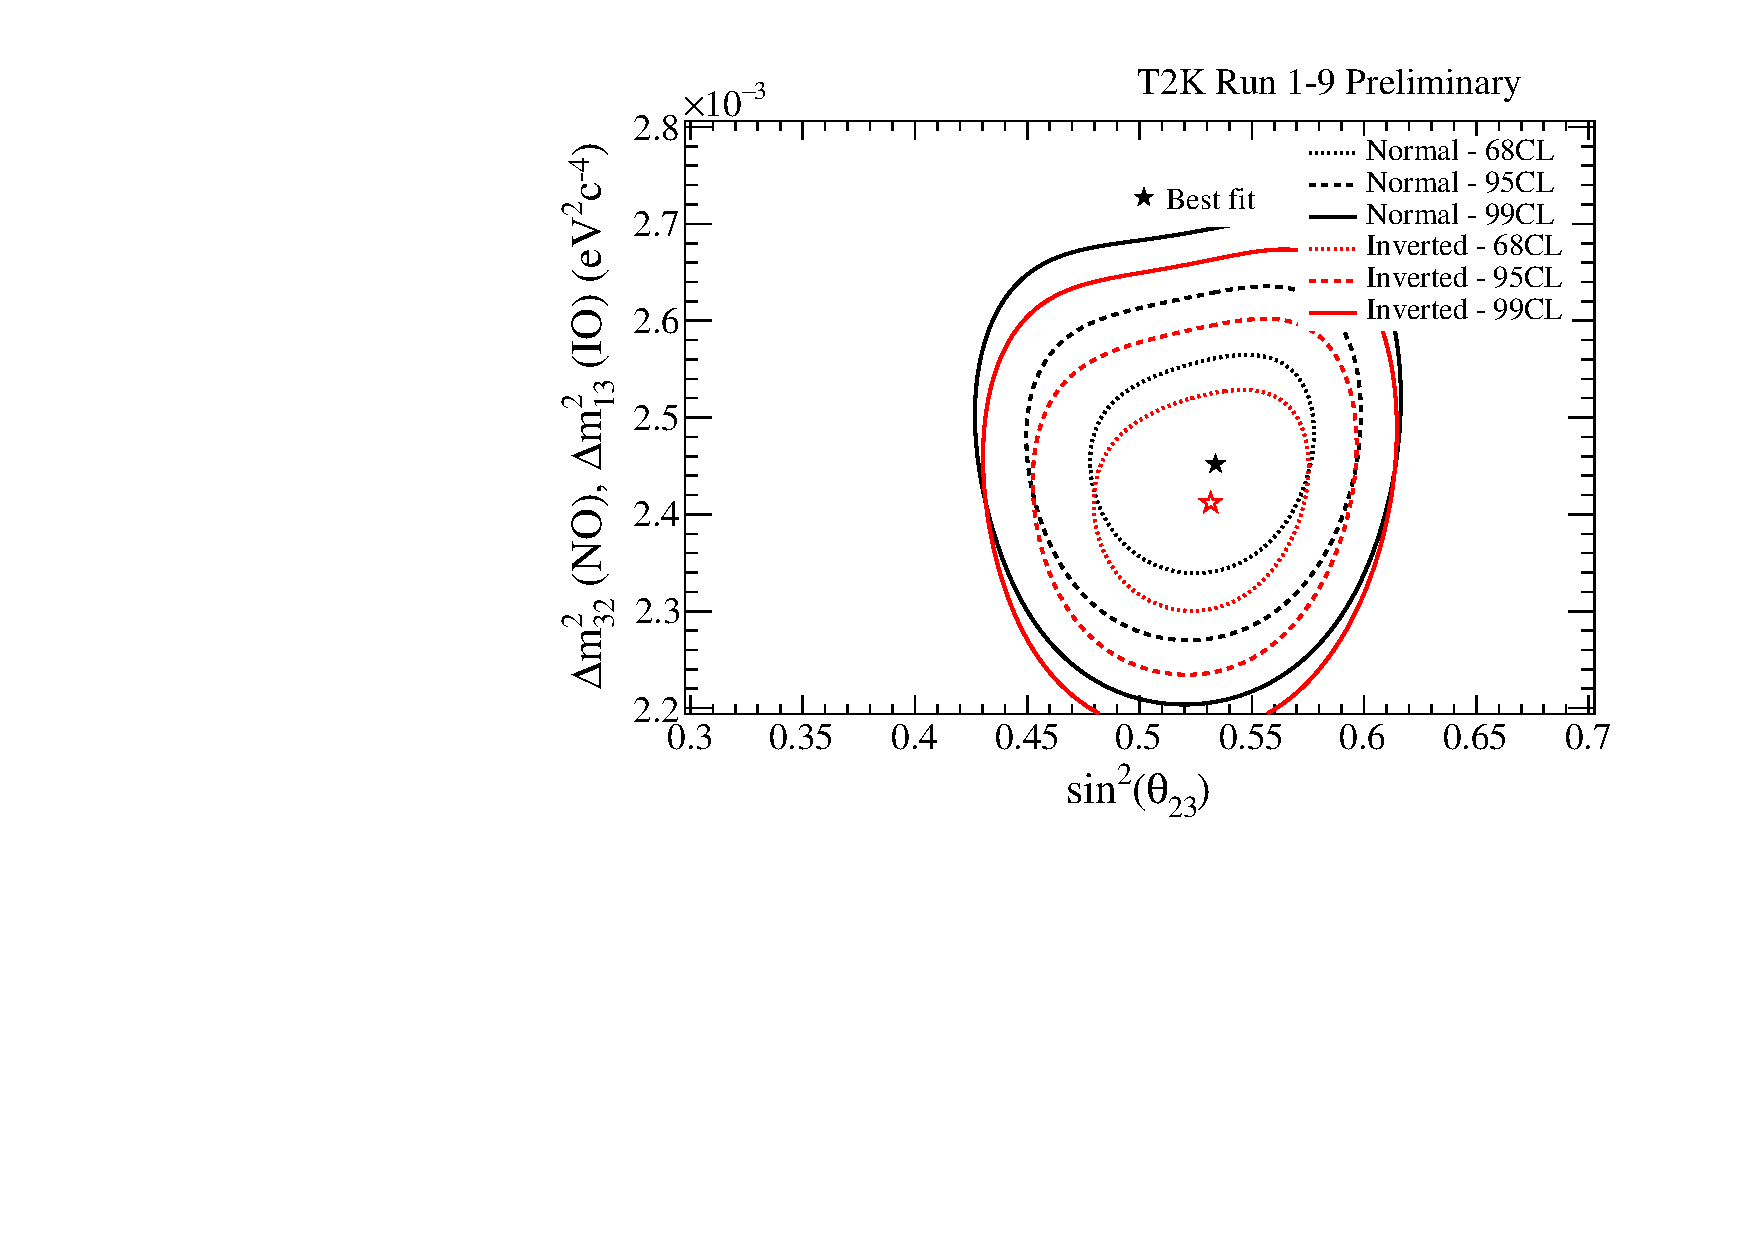
\includegraphics[width=0.45\textwidth]{images/data/3sigma/mixing23_dmsq23_data_reactor_global_3sigma}
	\caption {
		Contours at 68\%, 95\% and 99\% CL for \disappearance with reactor constraint. Normal and inverted hierarchy contours are independent. All 5 samples were used to produce these fits.
	}
	\label{fig:ssqth23_vs_dmsq23_data_3sigma}
\end{figure*}

\subsubsection{VALOR/MaCh3 comparison for \main}

The result for \main with reactor constraint is shown in fig.~\ref{fig:dcp_vs_ssqth23_data_group_compare_3sigma}.

\begin{figure*}[htb]
	\center
	\begin{subfigure}[b]{0.49\textwidth}
		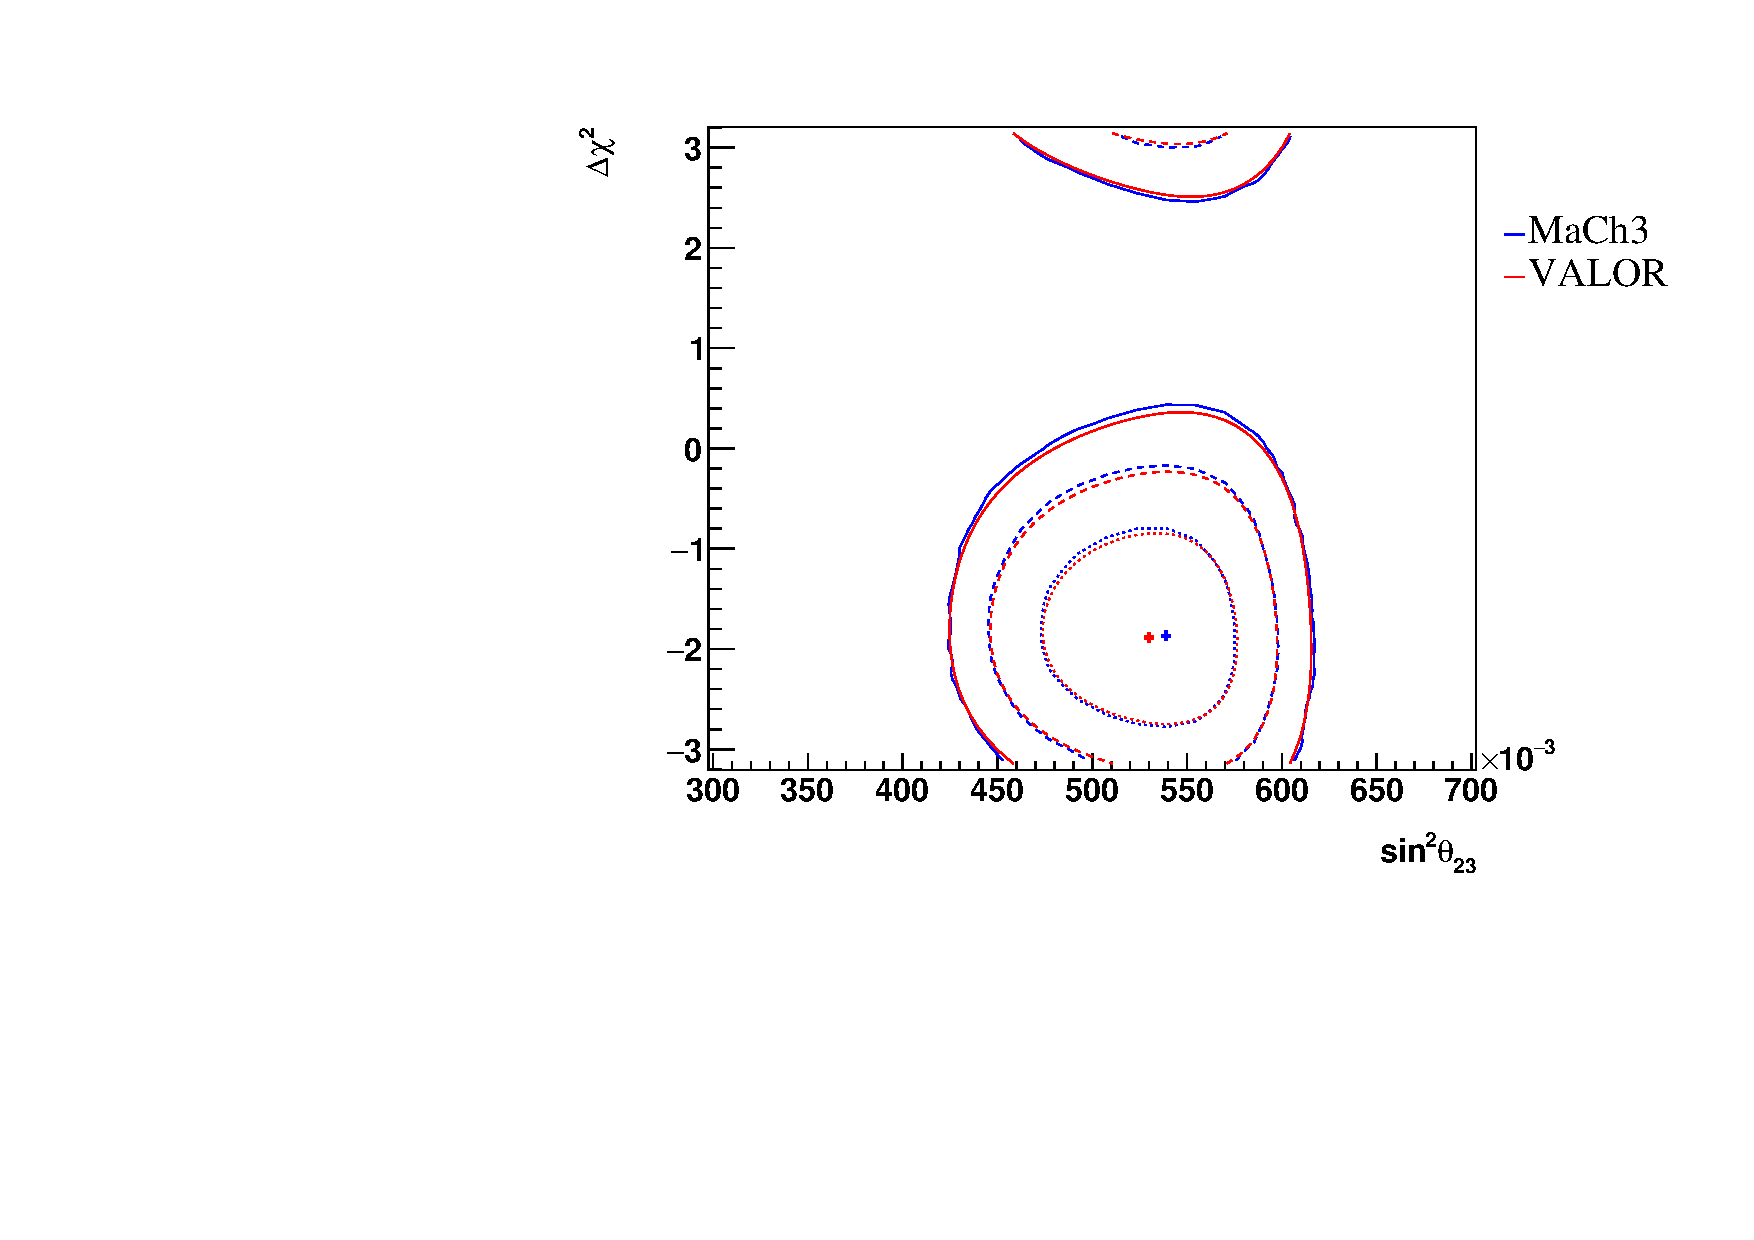
\includegraphics[width=0.9\textwidth]{images/data/group_comparison/3sigma/main_wrc_nh_data}
		\caption{\deltacp vs \ssqthtwothree NH with reactor constraint}
	\end{subfigure}
	\begin{subfigure}[b]{0.49\textwidth}
		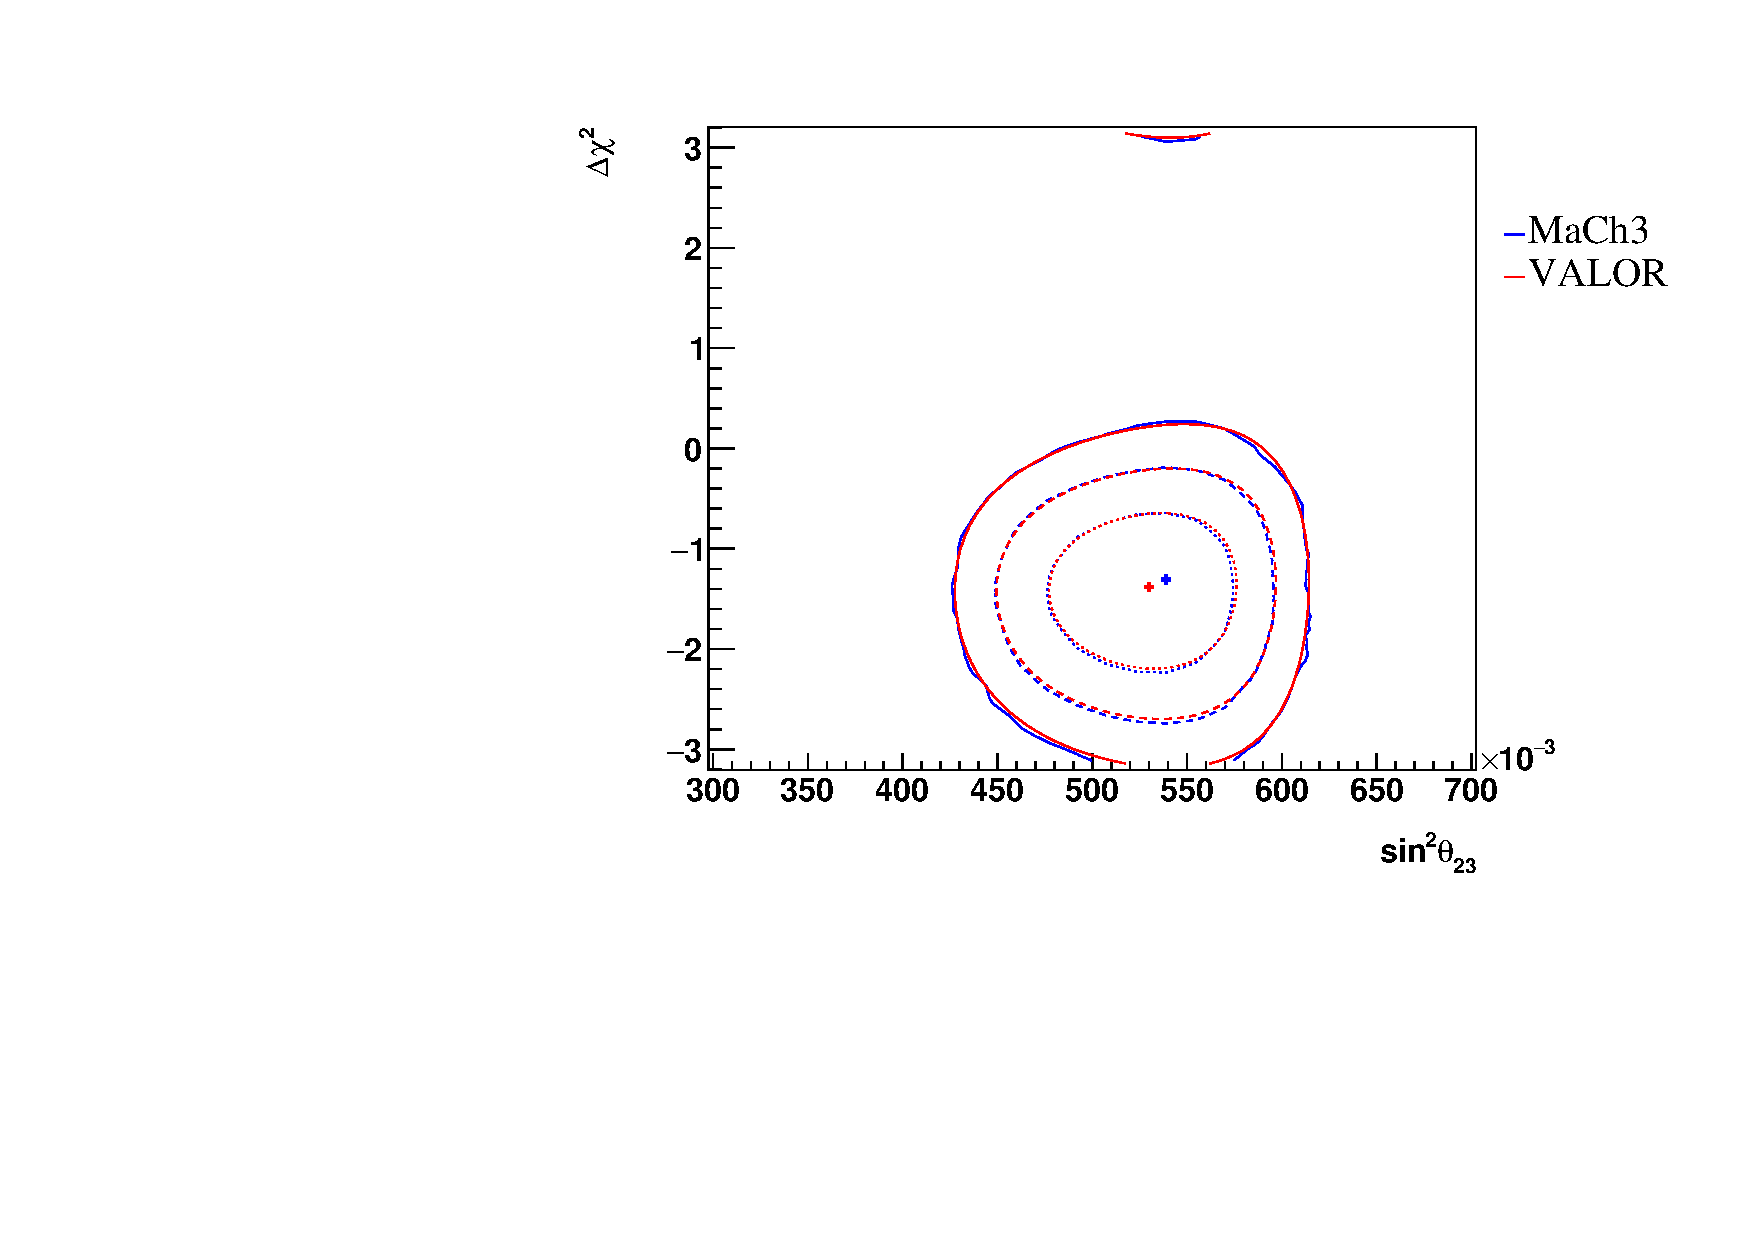
\includegraphics[width=0.9\textwidth]{images/data/group_comparison/3sigma/main_wrc_ih_data}
		\caption{\deltacp vs \ssqthtwothree IH with reactor constraint}
	\end{subfigure}
	\caption {
		Contours at 68\% and 90\% CL for \main with (top) and without (bottom) reactor constraint. Normal and inverted hierarchy contours are independent. All 5 samples were used to produce these fits.
	}
	\label{fig:dcp_vs_ssqth23_data_group_compare_3sigma}
\end{figure*}

\clearpage

\subsubsection{VALOR/MaCh3 comparison for \appearance}
In \cref{fig:ssqth13_vs_dcp_data_group_compare_3sigma} the result for \appearance with reactor constraint is shown.

\begin{figure*}[htb]
	\center
	\begin{subfigure}[b]{0.49\textwidth}
		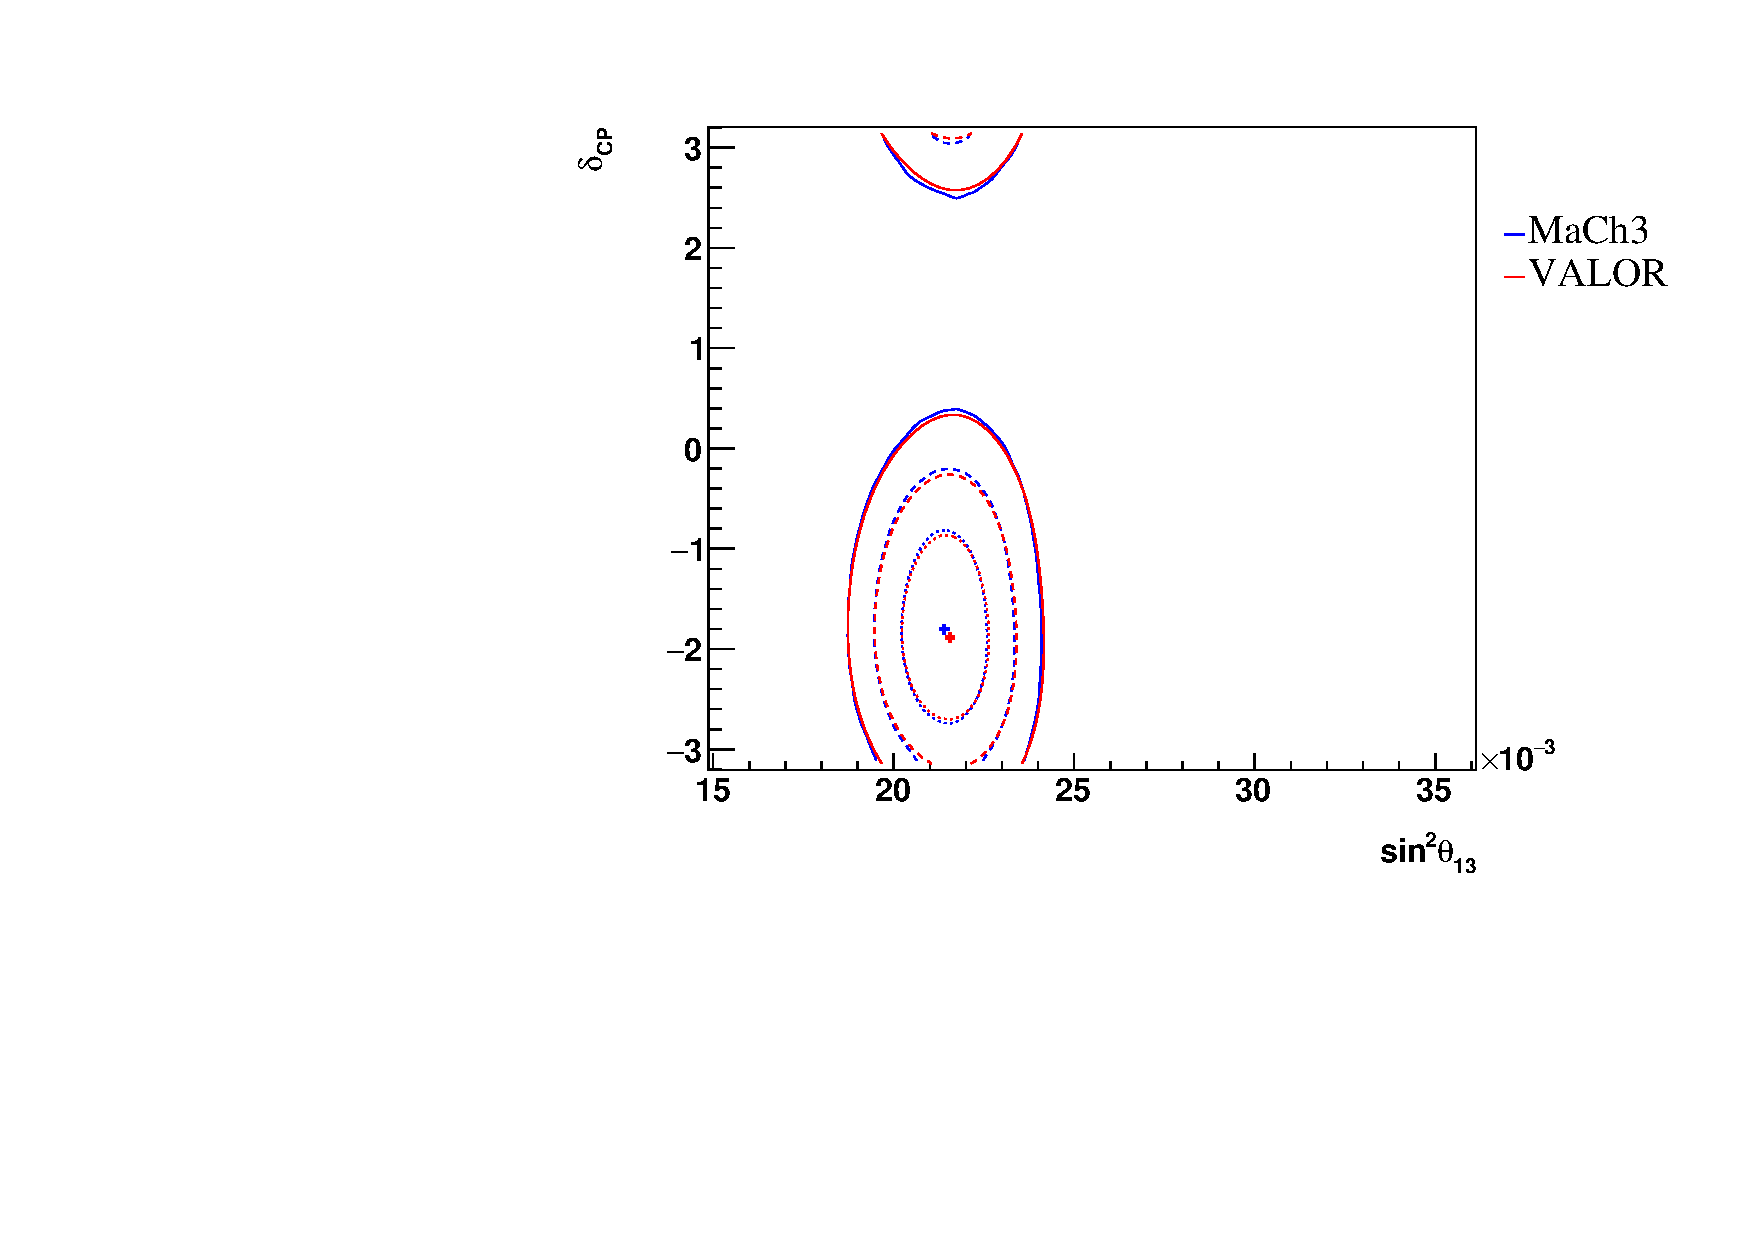
\includegraphics[width=0.9\textwidth]{images/data/group_comparison/3sigma/appearance_wrc_nh_data}
		\caption{\appearance NH with reactor constraint}
	\end{subfigure}
	\begin{subfigure}[b]{0.49\textwidth}
		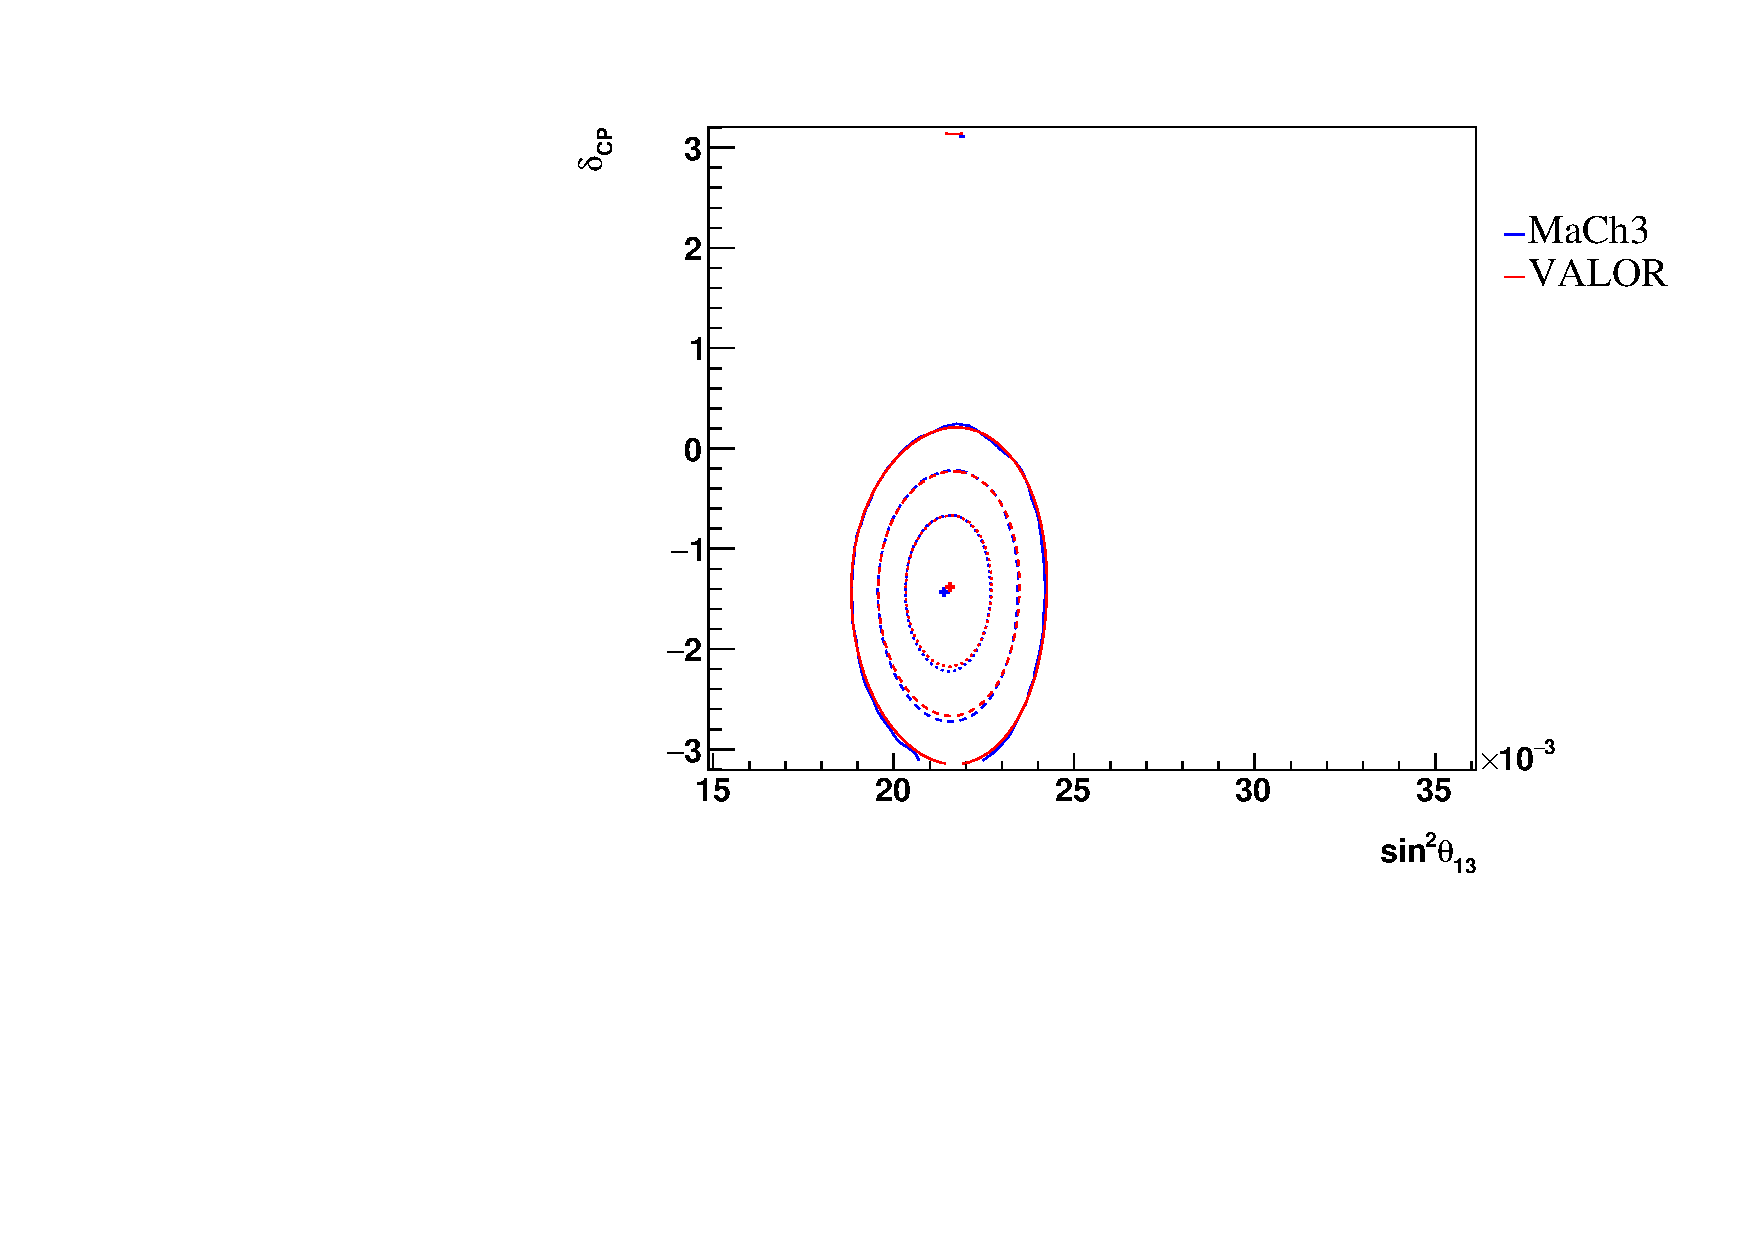
\includegraphics[width=0.9\textwidth]{images/data/group_comparison/3sigma/appearance_wrc_ih_data}
		\caption{\appearance IH with reactor constraint}
	\end{subfigure}
	\caption {
		Contours at 68\% and 90\% CL for \appearance with and without reactor constraint. Normal and inverted hierarchy contours are independent. All 5 samples were used to produce these fits.
	}
	\label{fig:ssqth13_vs_dcp_data_group_compare_3sigma}
\end{figure*}

\subsubsection{VALOR/MaCh3 comparison for \disappearance}

The result for \disappearance with reactor constraint is shown in fig.~\ref{fig:ssqth23_vs_dmsq_data_group_compare_3sigma}.

\begin{figure*}[htb]
	\center
	\begin{subfigure}[b]{0.49\textwidth}
		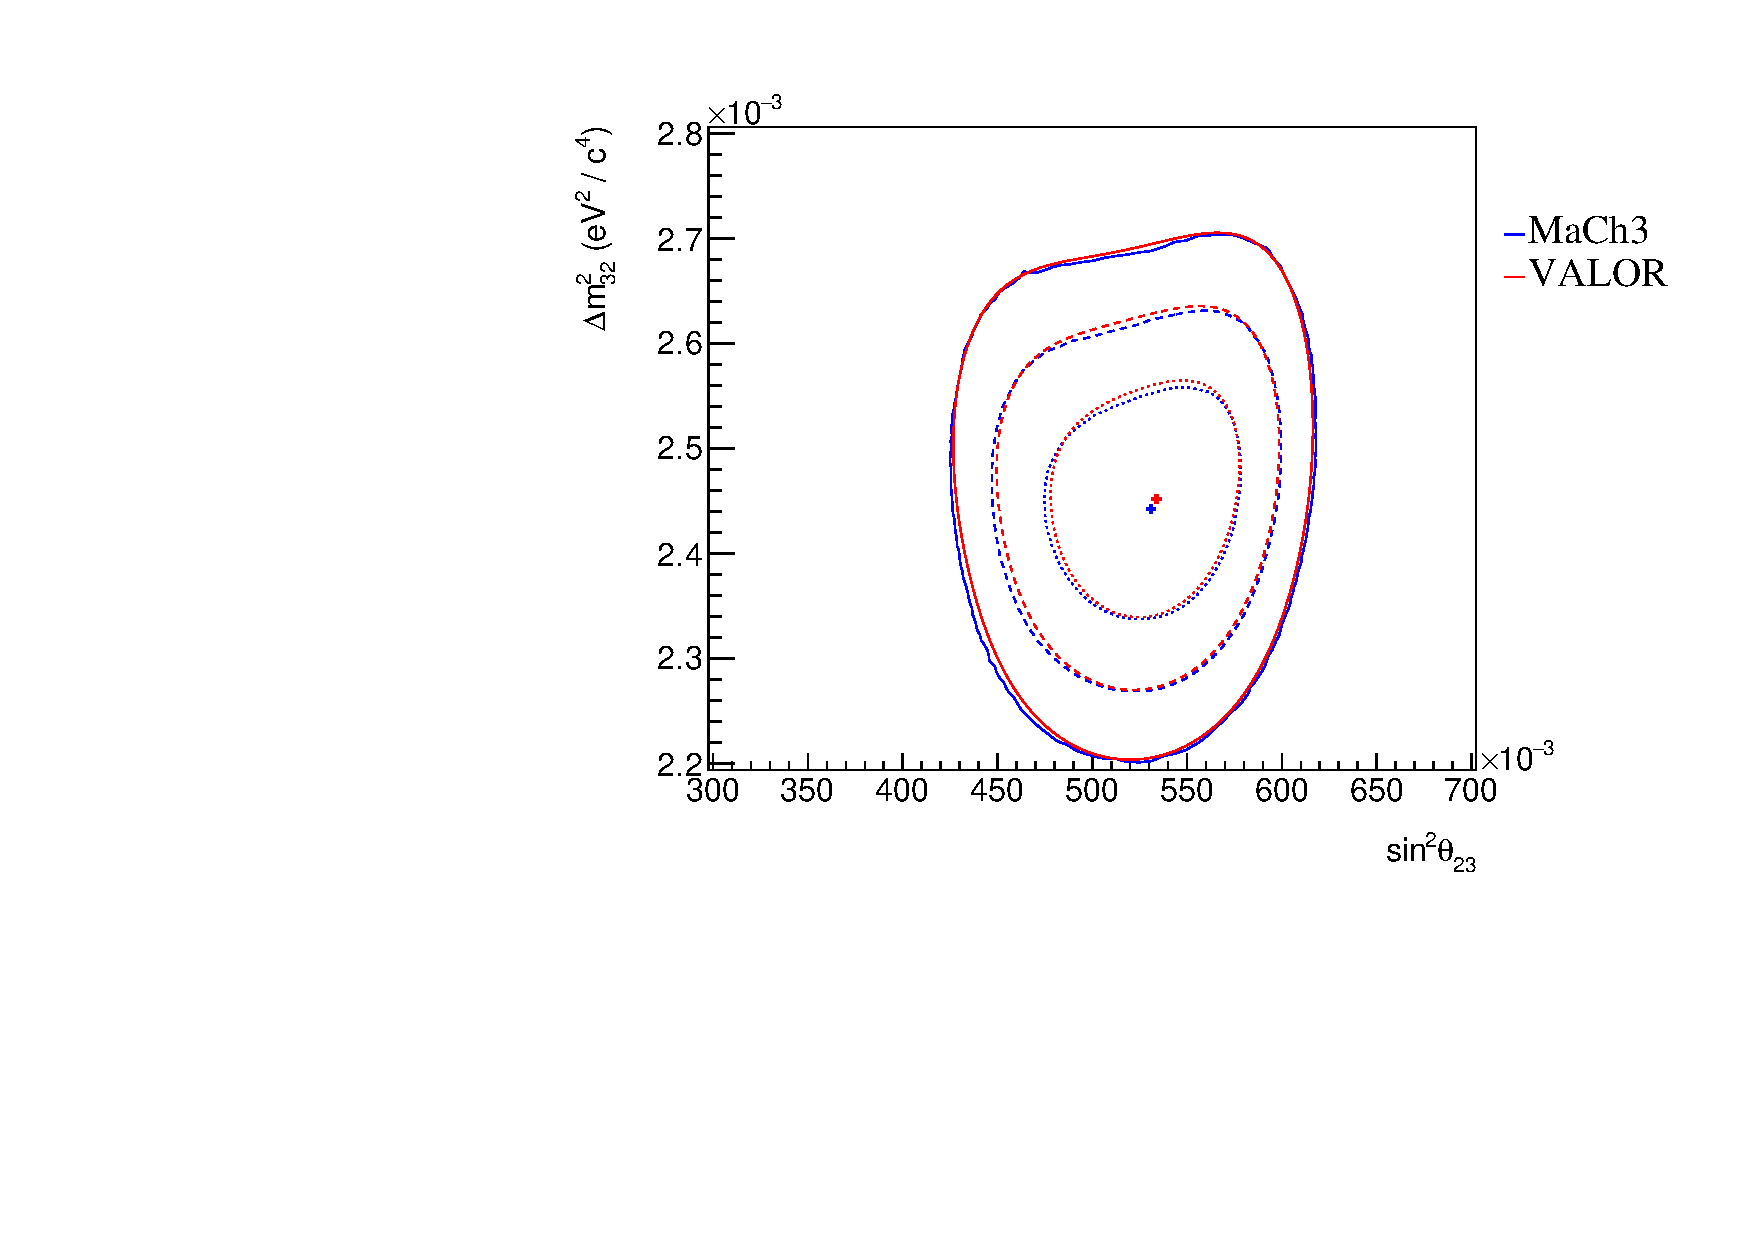
\includegraphics[width=0.9\textwidth]{images/data/group_comparison/3sigma/disappearance_wrc_nh_data}
		\caption{\disappearance NH with reactor constraint}
	\end{subfigure}
	\begin{subfigure}[b]{0.49\textwidth}
		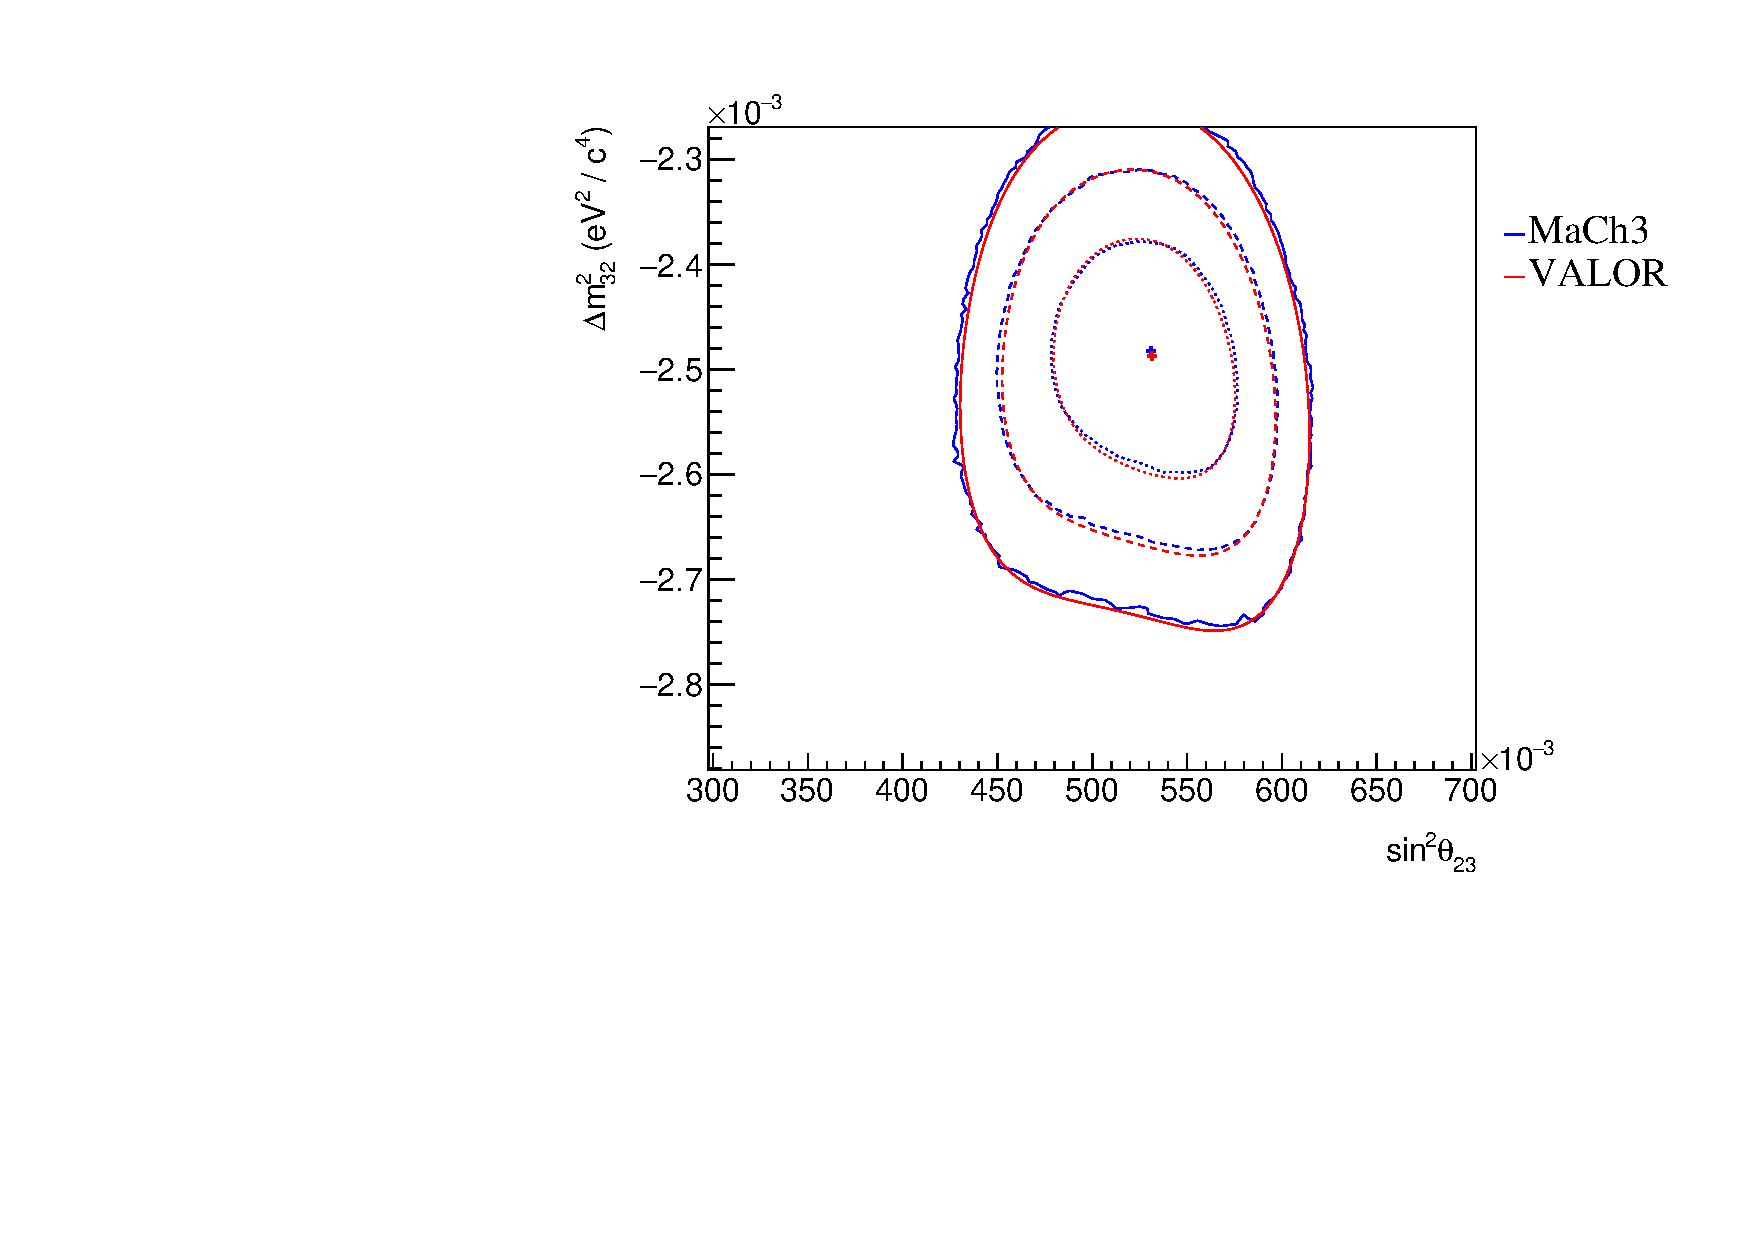
\includegraphics[width=0.9\textwidth]{images/data/group_comparison/3sigma/disappearance_wrc_ih_data}
		\caption{\disappearance IH with reactor constraint}
	\end{subfigure}
	\caption {
		Contours at 68\% and 90\% CL for \disappearance with (top) and without (middle) reactor constraint and comparison to p-theta reactor fit with $E_r-\theta$ templates (bottom). Normal and inverted hierarchy contours are independent. All 5 samples were used to produce these fits.
	}
	\label{fig:ssqth23_vs_dmsq_data_group_compare_3sigma}
\end{figure*}

\FloatBarrier
\clearpage
